\chapter{Vedic Mathematics}
%
The word “Veda” has this derivational meaning i.e. the fountain head and unlimited store-house of all knowledge. Vedic mathematics shows its application in fast calculations for multiplication, division, squaring, cubing, square root, cube root, trigonometry, log and exponential. The basic sutras and upa sutras in the Vedic Mathematics helps to do almost all the numeric computations in easy and fast manner. The ancient Indian Vedic mathematics is now currently employed in our global silicon chip technology for easier and faster calculations.

Vedic mathematics is part of four Vedas (books of wisdom). It is part of Sthapatya- Veda (book on civil engineering and architecture), which is an upa-veda (supplement) of Atharva Veda. It covers explanation of several modern mathematical terms including arithmetic, geometry (plane, co-ordinate), trigonometry, quadratic equations, factorization and even calculus \cite{r1}.

His Holiness Jagadguru Shankaracharya Bharati Krishna Teerthaji Maharaja (1884-1960) comprised all this work together and gave its mathematical explanation while discussing it for various applications. Swamiji constructed 16 sutras (formulae) and 13 Upa sutras (sub formulae) after extensive research in Atharva Veda. Obviously these formulae are not to be found in present text of Atharva Veda because these formulae were constructed by Swamiji himself. Vedic mathematics is not only a mathematical wonder but also it is logical, due to which Vedic mathematics has such a degree of eminence which cannot be disapproved. Having these phenomenal characteristic, Vedic mathematics has already crossed the boundaries of India and has become a leading topic of research in abroad. VM deals with several basic as well as complex mathematical operations. Especially, methods of basic arithmetic are extremely simple and powerful.

%Vedic mathematics is mainly based on 16 Sutras (or aphorisms) and 13 upa sutras dealing with various branches of mathematics like arithmetic, algebra, geometry etc. These Sutras along with their brief meanings are enlisted below alphabetically.
Entire mechanics of Vedic mathematics is based on 16 sutras – formulas and 13 up-sutras meaning – corollaries which are enlisted below.\\
Sutras
\begin{enumerate}
  \item Ekadhikena Purvena
  \item Nikhilam Navatascharamam Dashatah
  \item Urdhva-tiryagbhyam
  \item Paravartya Yojayet
  \item Shunyam Samyasamucchaye
  \item Anurupye Sunyamanyat
  \item Sankalana vyavakalanabhyam
  \item Puranaprranabhyam
  \item Calana – Kalanabhyam
  \item Yavadunam
  \item Vyastisamashtih
  \item Sheshanynkena Charmena
  \item Sopantyadvayamantyam
  \item Ekanyunena Purvena
  \item Ginitasamucchayah
  \item Gunaksamucchayah
\end{enumerate}

Up-sutras
\begin{enumerate}
  \item Anurupyena
  \item Shishyate Sheshsamjnah
  \item Adyamadye Nantyamantyena
  \item Kevalaih Saptakam Gunyat
  \item Vestanam
  \item Yavadunam Tavadunam
  \item Yavadunam Tavadunikutya Varganka ch Yojayet
  \item Antyayordhshakepi
  \item Antyatoreva
  \item Samucchayagunitah
  \item Lopanasthapanabhyam
  \item Vilokanam
  \item Gunitasamucchyah Samucchayagunitah
\end{enumerate}

These methods and ideas can be directly applied to trigonometry, plain and spherical geometry, conics, calculus (both differential and integral), and applied mathematics of various kinds. As mentioned earlier, all these Sutras were reconstructed from ancient Vedic texts early in the last century. %Many Sub-sutras were also discovered at the same time, %which are not discussed here.

The beauty of Vedic mathematics lies in the fact that it reduces the otherwise cumbersome-looking calculations in conventional mathematics to a very simple one. This is so because the Vedic formulae are claimed to be based on the natural principles on which the human mind works. This is a very interesting field and presents some effective algorithms which can be applied to various branches of engineering such as computing and digital signal processing.

%The multiplier architecture can be generally classified into three categories. First is the serial multiplier which emphasizes on hardware and minimum amount of chip area. Second is parallel multiplier (array and tree) which carries out high speed mathematical operations. But the drawback is the relatively larger chip area consumption. Third is serial- parallel multiplier which serves as a good trade-off between the times consuming serial multiplier and the area consuming parallel multipliers.

\section{Vedic Multiplication}

The proposed Vedic multiplier is based on the Vedic multiplication formulae (Sutras). These Sutras have been traditionally used for the multiplication of two numbers in the decimal number system. In this work, we apply the same ideas to the binary number system to make the proposed algorithm compatible with the digital hardware. In Vedic mathematics there are 3 methods to implement multiplication. Out of three there is
one generic method which can be applied to all cases whereas other two are for special cases which are simpler to deal with. Main algorithm of vedic multiplication is discussed below :
%Vedic multiplication based on some algorithms, some are discussed below:

\subsection{Urdhva triyakbhyam Sutra}

Urdhva tiryakbhyam Sutra is a general multiplication formula applicable to all cases of multiplication. It literally means “Vertically and Crosswise”. These Sutras have been traditionally used for the multiplication of two numbers in the decimal number system. In this work, we apply the same ideas to the binary number system to make the proposed algorithm compatible with the digital hardware. It is based on a novel concept through which the generation of all partial products can be done with the concurrent addition of these partial products. The algorithm can be generalized for n x n bit number. Since the partial products and their sums are calculated in parallel, the multiplier is independent of the clock frequency of the processor. The Multiplier based on this sutra has the advantage that as the number of bits increases, gate delay and area increases very slowly as compared to other conventional multipliers. The 4x4 multiplication using urdhva triyakbhyam is shown in Figure \ref{lined} and \ref{eqa}.

\begin{figure}[h]
\begin{center}
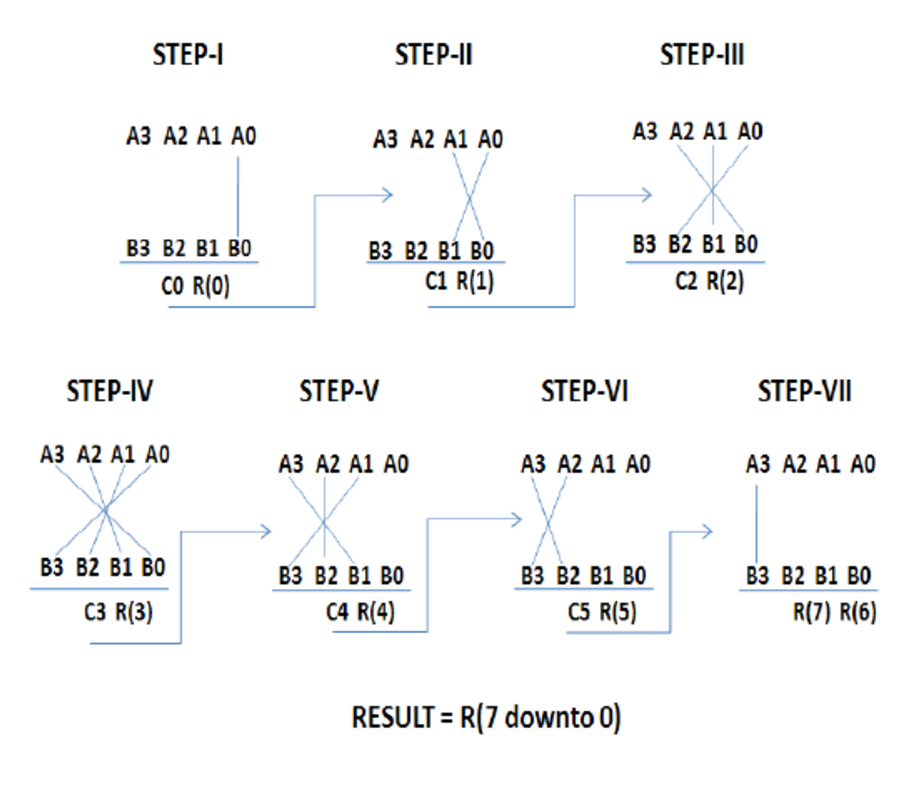
\includegraphics[width=3.5in]{linedia.eps}
\caption{4x4 Multiplication method of Urdhva-Tiryakbhyam \cite{r8}.} \label{lined}
\end{center}
\end{figure}
\pagebreak

\begin{figure}[h]
\begin{center}
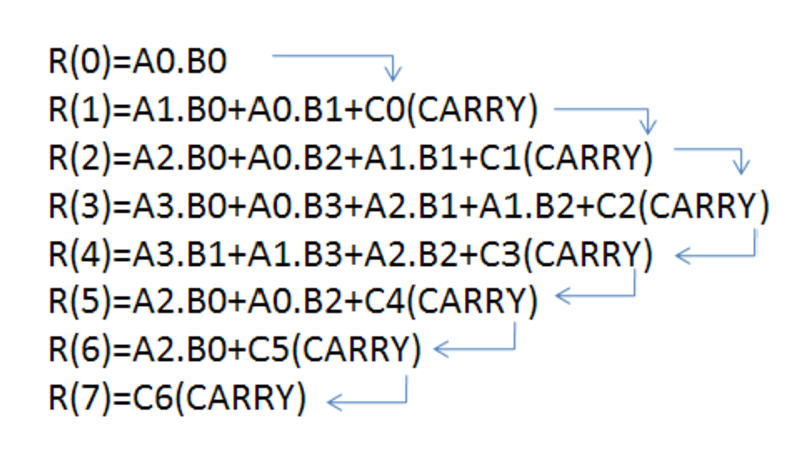
\includegraphics[width=3.5in]{equations.eps}
\caption{Equations used for designing a 4x4 Vedic-Multiplier \cite{r8}.} \label{eqa}
\end{center}
\end{figure}



%%%%%%%%%%%%%%%%%%%%%%%%%%%%%%%%%%%%%%%%%%%%%%%%%%%%%%%%%%%%%%%
%\section{Comparison with IR communication}
%
%The differences between VLC and infrared communication are listed in Table 1.
%
%%%%%%%%%%%%%%%%%%%%%%%%%%%%%%%%%%%%%%%%%%%%table
%\begin{table}[h]
%\caption{Comparison of short-range wireless communication technologies. (FIR: fast infrared, VFIR: very fast infrared) \cite{r15}.}
%\centering
%
%\begin{tabular}{|p{1in}|p{2in}|p{2in}|}
%%%\begin{tabular}{|c|c|c|}
%
%%\caption{Comparison of short-range wireless communication technologies (FIR fast infrared, VFIR very fast infrared).}
%  \hline
%  % after \\: \hline or \cline{col1-col2} \cline{col3-col4} ...
%  Parameters & Visible Light Communication & Infrared Communication \\
%  \hline
%  Data Rate & $>$100Mb/s possible (LED dependent)& 4Mb/s(FIR),16 Mb/s (VFIR) \\
%  \hline
%  Status & Research and standardization in IEEE & Standardization (IrDA) \\
%  \hline
%  Distance & ~meters & ~3 meters \\
%  \hline
%  Regulation & No & No \\
%  \hline
%  Security & Good & Good \\
%  \hline
%  Carrier wavelength (frequency) & 380$~$780 nm visible light (multiple wavelengths) & 850 nm infrared \\
%  \hline
%  Services & Communication, illumination & Communication \\
%  \hline
%  Noise Source & Sun light, Other illumination & Ambient light \\
%  \hline
%  Environmental & Daily usage Eye safe (visible) & Eye safe for low power (invisible) \\
%  \hline
%  Applications & Indoor vehicular communication, Optical ID & Remote control, Point to point connection \\
%  \hline
%\end{tabular}
%\label{table:comp}
%\end{table}
%
%%%%%%%%%%%%%%%%%%%%%%%%%%%%%%%%%%%%%%%%%%%%%%end table
\begin{tabular}{|c|c|}
  \hline
  % after \\: \hline or \cline{col1-col2} \cline{col3-col4} ...
  1 & 2 \\
  \hline
  3 & 4 \\
  \hline
\end{tabular}
%

